\documentclass[12pt]{article}%
\usepackage{amsfonts}
\usepackage{fancyhdr}
\usepackage{comment}
\usepackage[a4paper, top=2.5cm, bottom=2.5cm, left=2.2cm, right=2.2cm]%
{geometry}
\usepackage{times}
\usepackage{graphicx}

\usepackage{hyperref}

\usepackage{amssymb}
\usepackage{graphicx}%

\begin{document}

\title{PODB - Assignment 1}
\author{Ayush Sekhari}
\date{\today}
\maketitle

\section{Question 1}
\subsection{Introduction}
I am making the ER model for Hostel Management (Hostel = Enterprise).
The ER model of the database can be found in figure \ref{fig:er}. It has been included in the file ER1.png in the zip archive that I uploaded. 

\begin{figure}
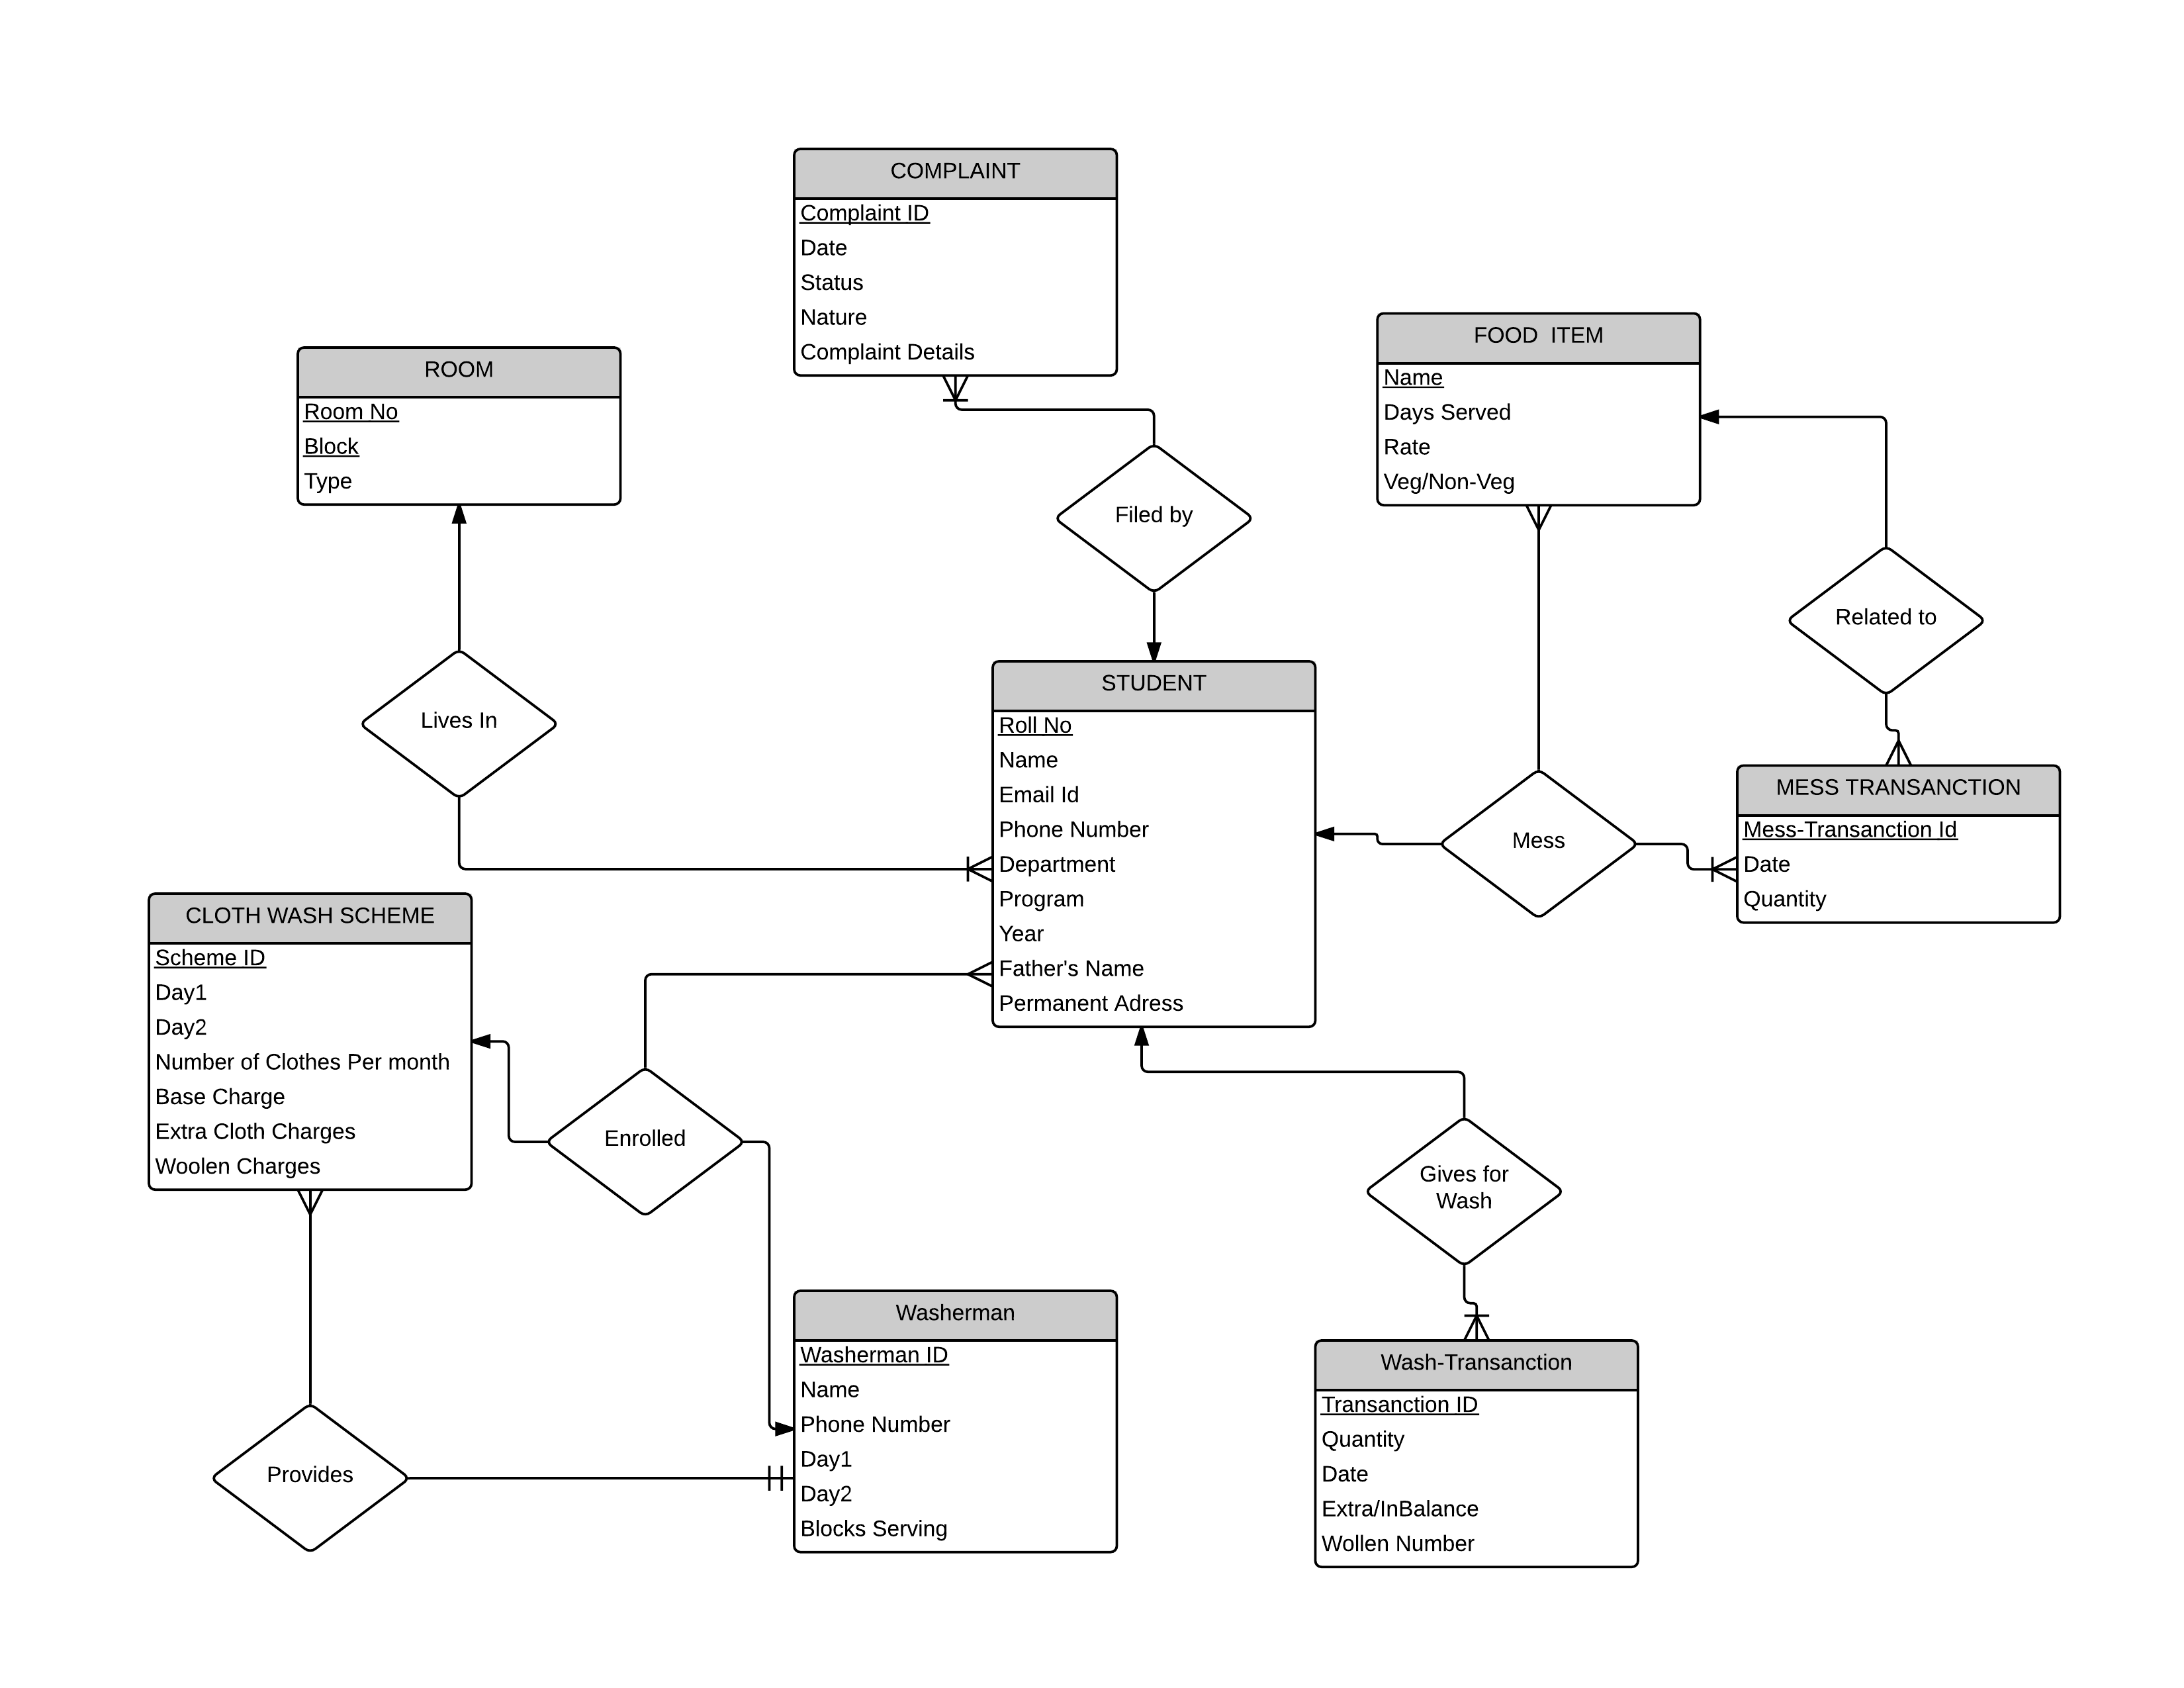
\includegraphics[width=\textwidth]{ER1.png}
\label{fig:er}
\caption{ER model for Hostel Management System}
\end{figure}

\subsection{Design Points}
\begin{enumerate}
\item Student is the central entity. 
\item Students can file multiple complaints. Each complaint has to be filed by some student only. 
\item Each student has a room. There may be multiple students in a room. A room may be empty. 
\item Student has to agree on some cloth wash scheme with a washerman. Each student can agree with only one washerman on only one scheme.
\item Students can take extras in the mess. These transactions are recorded in the mess transactions. A student can have multiple transactions for some food items. Every transaction is for some student for some food item. 
\item Student can have Wash-transactions. Each such transaction is for a student. 
\end{enumerate}

\subsection{Relation Schema}
The tables shown in figure \ref{fig:erschema} can be used to store data in the database. Here, all the tables are in 3NF form. It has also been included in the file ER1Schema.png in the zip archive that I uploaded. 

\begin{figure}
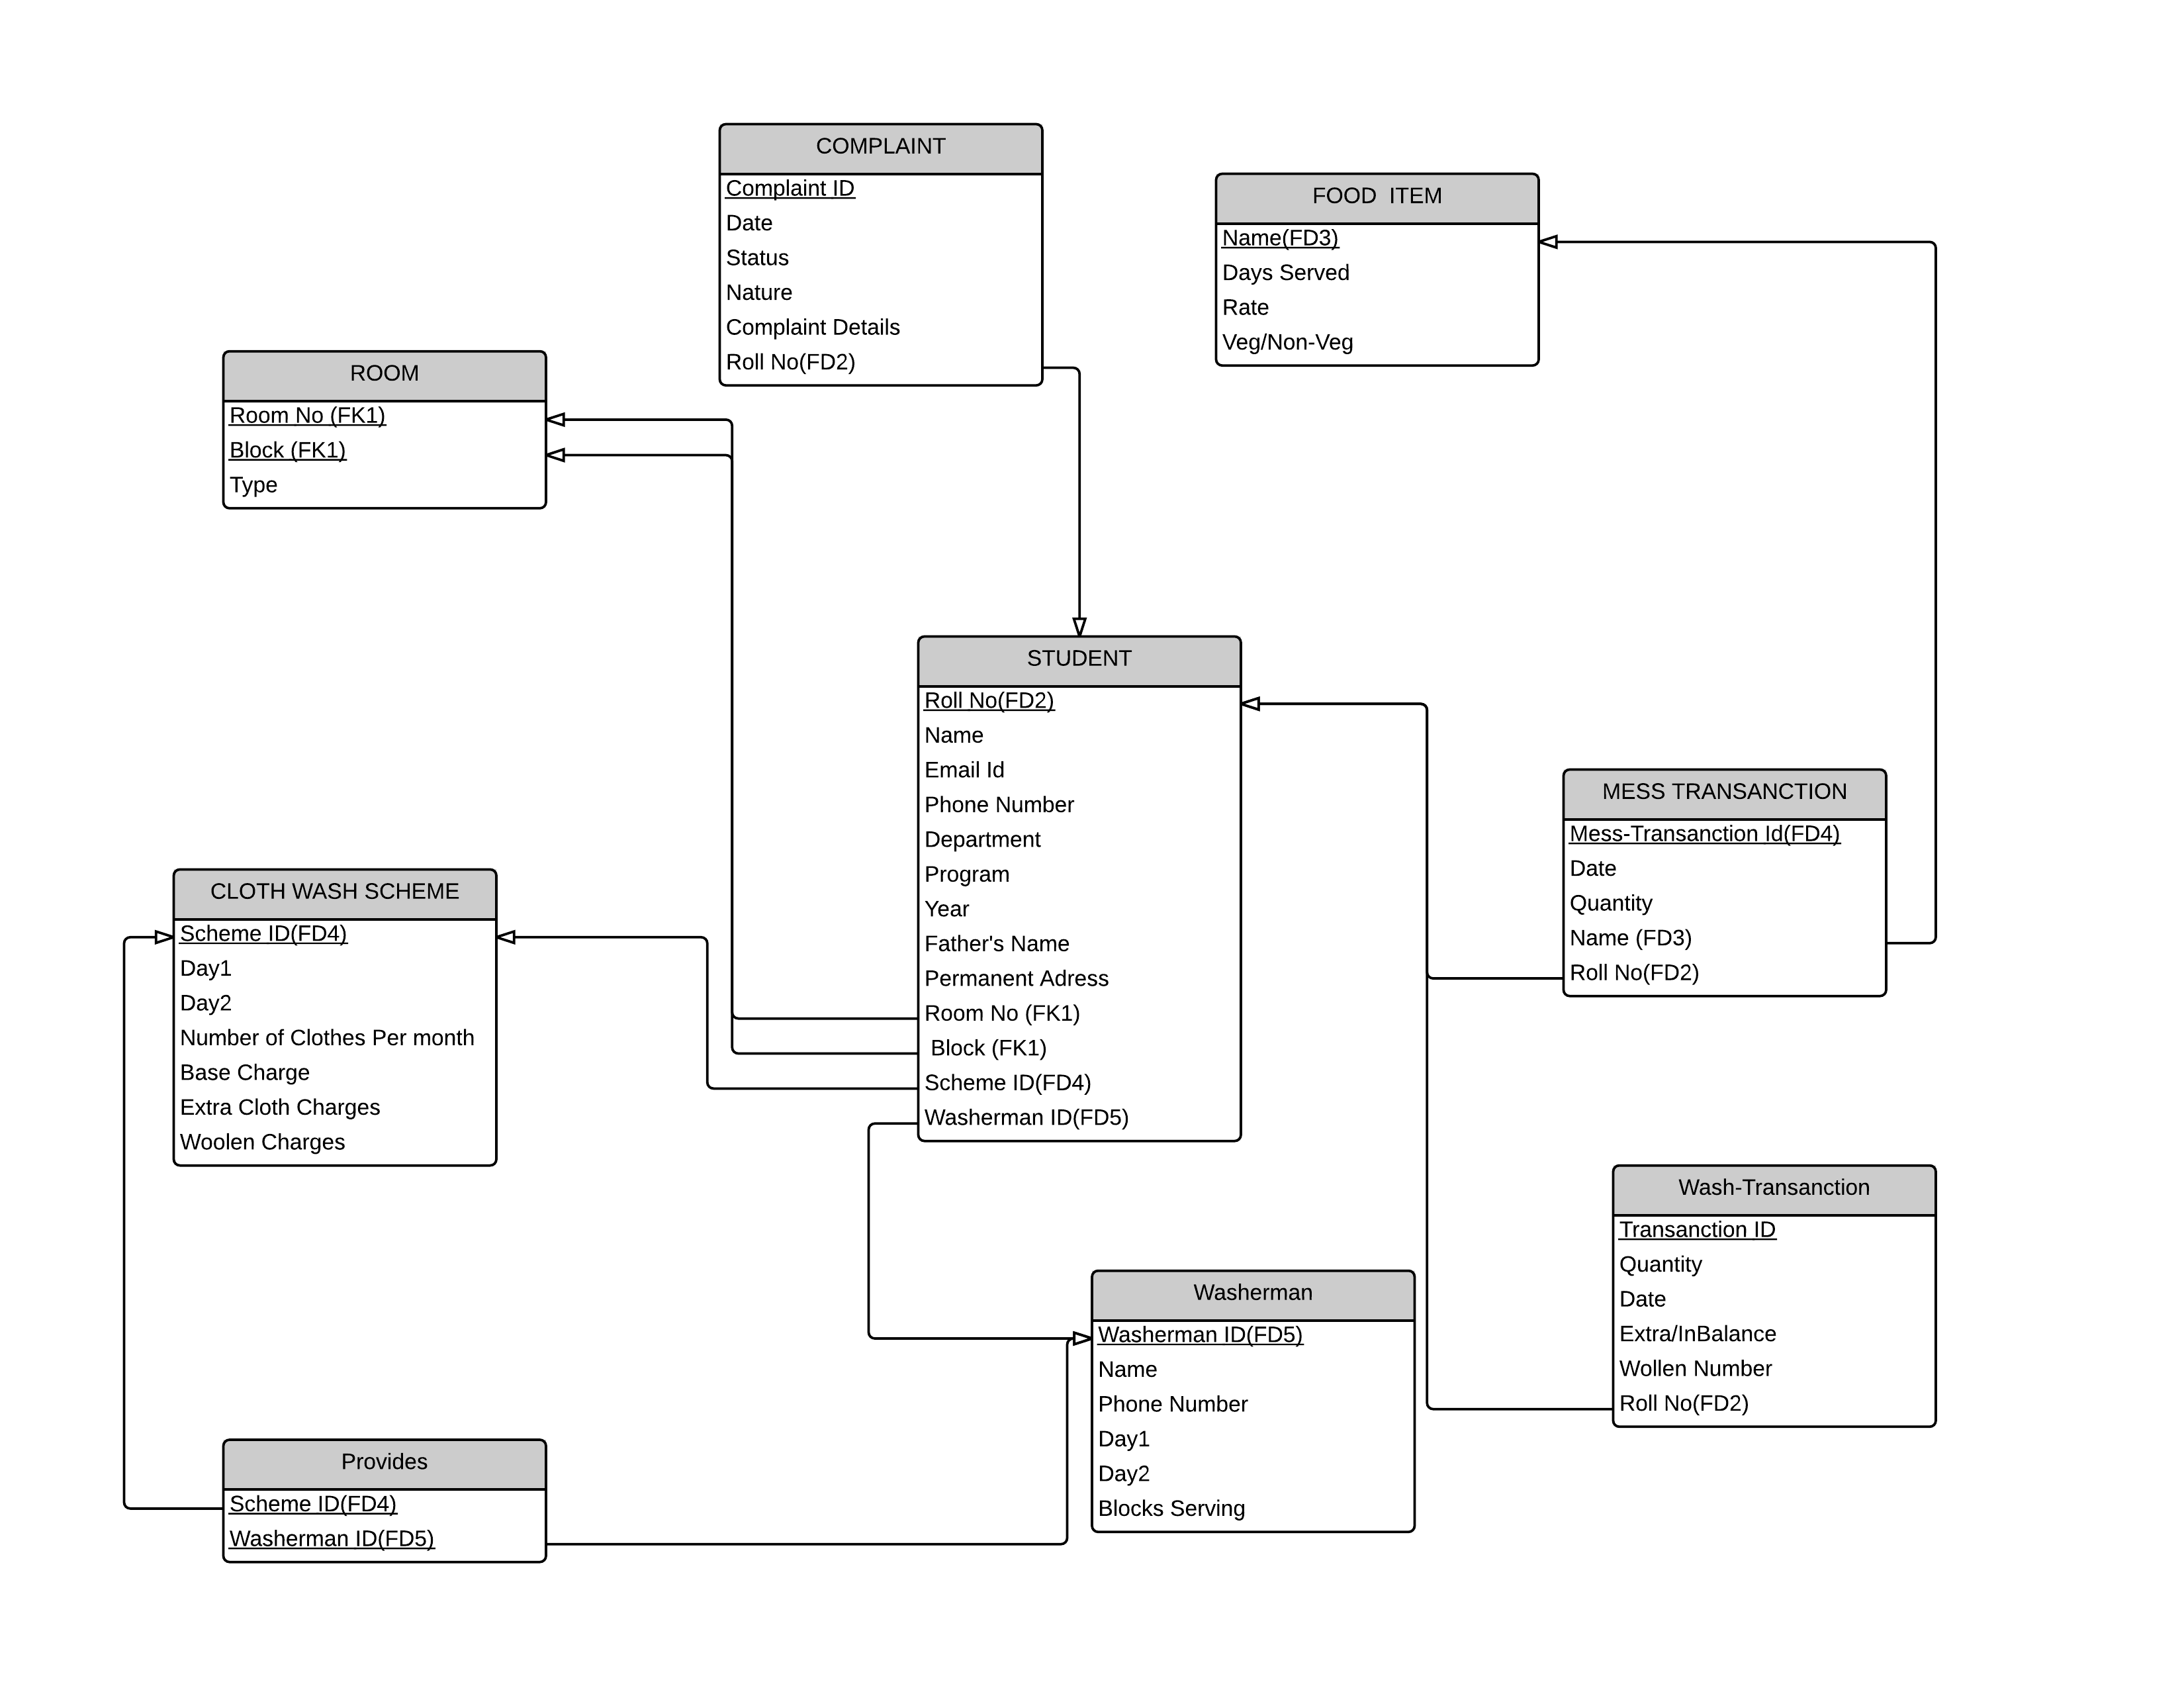
\includegraphics[width=\textwidth]{ER1Schema.png}
\label{fig:erschema}
\caption{Database schema for Hostel Management System}
\end{figure}

\section{Question 2}
\subsection{ER Model}
The ER model of the IIT Kanpur Academic Model  can be found in figure \ref{fig:er2}.
It has also been included in the file ER2.png in the zip archive that I uploaded. 

\begin{figure}
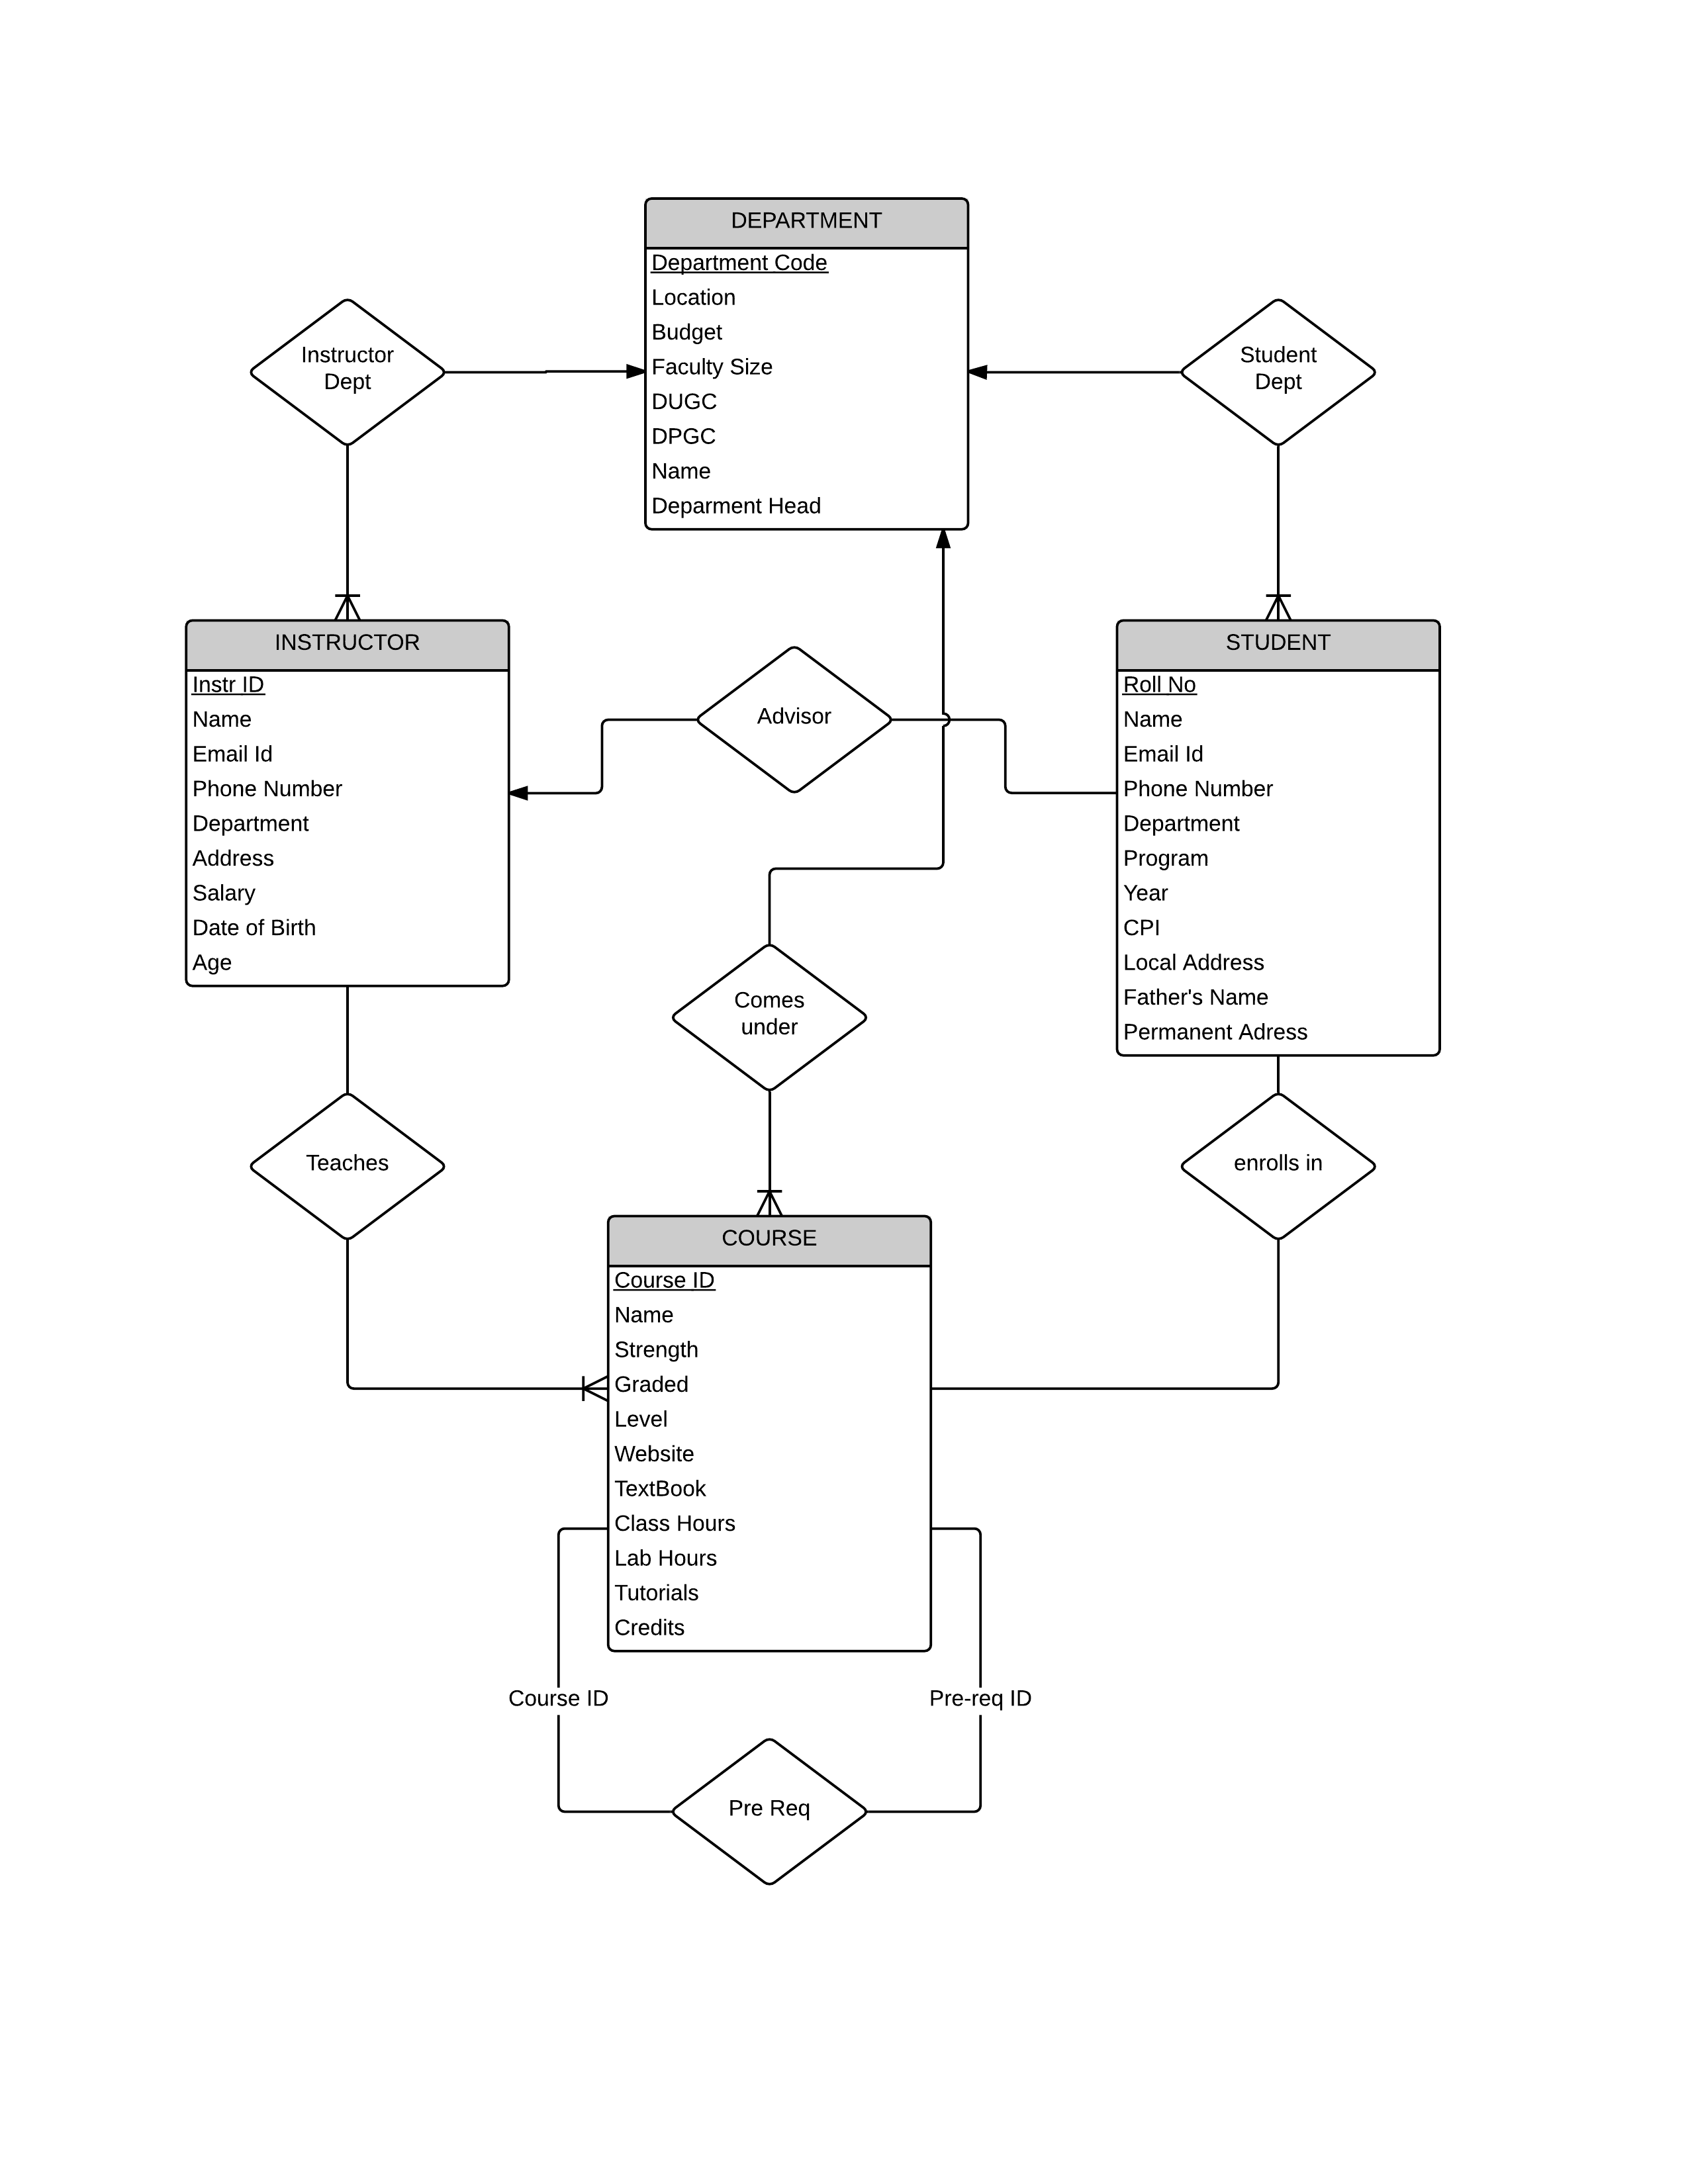
\includegraphics[width=\textwidth]{ER2.png}
\label{fig:er2}
\caption{ER model for IIT Kanpur Academic System}
\end{figure}

\subsection{Relation Schema}
The tables shown in figure \ref{fig:er2schema} can be used to store data in the database. It has also been included in the file ER2Schema.png in the zip archive that I uploaded. 

\begin{figure}
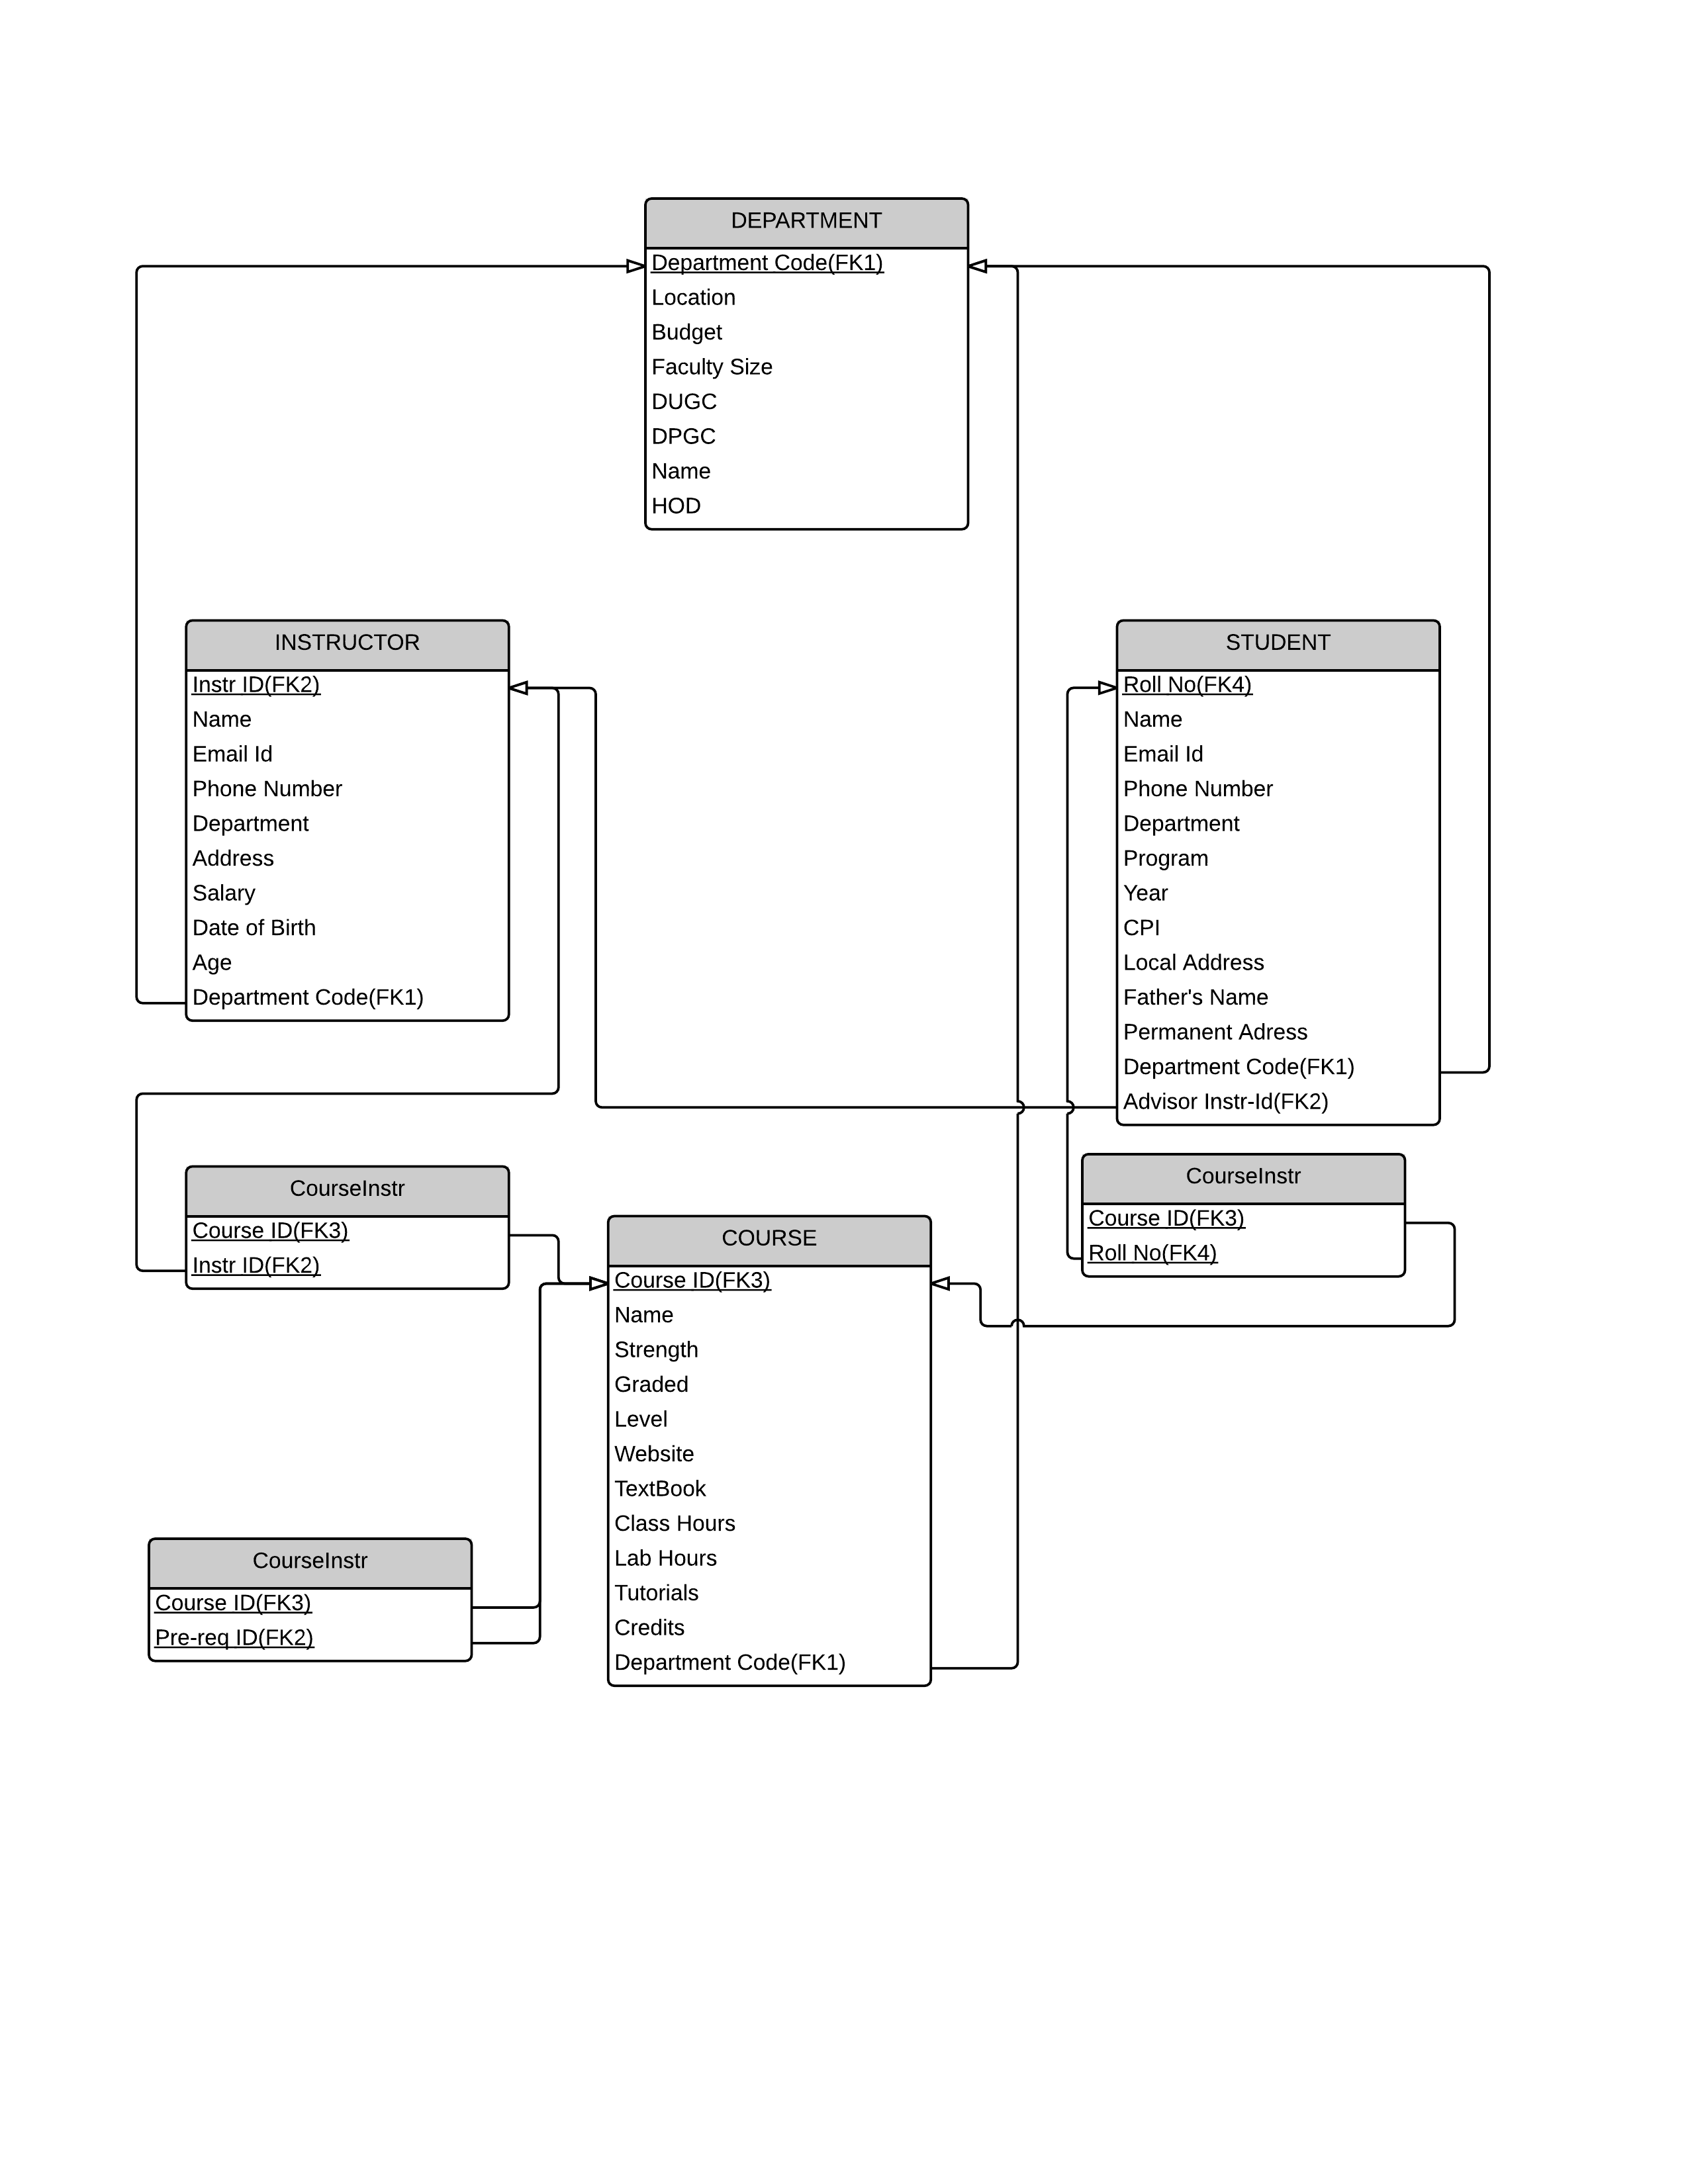
\includegraphics[width=\textwidth]{ER2Schema.png}
\label{fig:er2schema}
\caption{Database Schema for IIT Kanpur Academic System}
\end{figure}

\subsection{Trivial Dependencies}
A lot of trivial dependencies can be made and exist. Some of them are as follows : 
\begin{itemize}
\item Roll No, Name $\rightarrow$ Name (In relation STUDENT)
\item Name , Email Id $\rightarrow$ Name (In relation INSTRUCTOR)
\end{itemize}

Since, we can make as many trivial dependencies as we want, making and dealing with them is useless. 

\subsection{Fully Functional Dependencies}
In the ER model and relation schema that I have made, some fully functional dependencies are as follows:
\begin{itemize}
\item All the attributes are full-functionally dependent on singleton candidate keys. Eg. 
\begin{itemize}
\item Department Code $\rightarrow$ HOD (in relation DEPARTMENT)
\item Instr ID $\rightarrow$ Name (in relation INSTRUCTOR)
\item Course Name $\rightarrow$ Credits (in relation COURSE)
\end{itemize}
\item Class House , Lab Hours , Tutorials $\rightarrow$ Credits (in relation COURSE)
\item Local Address , Name $\rightarrow$ Roll No (in relation STUDENT, assuming that we do not have two students with same name sharing a room)
\item Name , Fathers Name , Permanent Address $\rightarrow$ Roll No
\item Date of Birth , Address , Department $\rightarrow$ Name , Phone Number , Email ID (in relation INSTRUCTOR , assuming that we do not have multiple prof. family with any two in the same department)
\end{itemize}
There may exists more fully functional dependencies in the actual IIT Kanpur academic database model. 
In general, whenever we have non-singleton candidate keys, We have fully functional dependencies there for all the attributes, as no subset of it would determine all the attributes. 
\subsection{Transitive Dependencies}
In the ER model and relation schema that I have made, some transitive dependencies are as follows:
\begin{itemize}
\item HOD $\rightarrow$ Department Code , Department Code $\rightarrow$ Budget (in relation DEPARTMENT)
\item DUGC $\rightarrow$ Name , Name $\rightarrow$ HOD (in relation DEPARTMENT) 
\end{itemize}
There may exists more transitive dependencies in the actual IIT Kanpur academic database model.
In general, whenever we have multiple candidate keys, We have fully transitive dependencies there.

\subsection{Multivalued dependencies}
We have some multivalued dependencies in the database design here. Eg :
\begin{itemize}
\item Name $\twoheadrightarrow$ Salary (in relation INSTRUCTOR)
\item Name $\twoheadrightarrow$ Program (in relation STUDENT)
\item Name $\twoheadrightarrow$ CPI (in relation STUDENT)
\item Stregth $\twoheadrightarrow$ Level (in relation COURSE)
\item Name $\twoheadrightarrow$ Date of Birth (in relation INSTRUCTOR)
\end{itemize}
There may exists more multivalued dependencies in the actual IIT Kanpur academic database model.

\begin{figure}
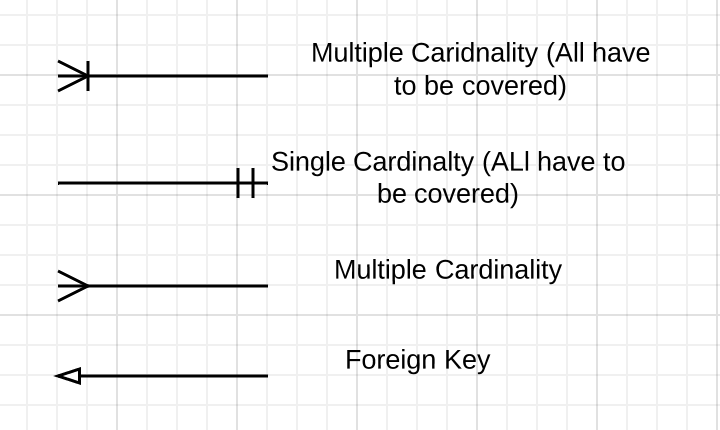
\includegraphics{symbols.png}
\label{fig:er2schema}
\caption{Standard Symbols and connectives in ER models and Schemas}
\end{figure}
\end{document}
